% Engineering Design: c-Field Modulator/Detector Prototype
% for DFD Communication Demonstration
%
% Supporting Patent 14: U.S. Provisional Application No. 63/865,293
% Gary Alcock, 2025--2026
%
\documentclass[11pt,letterpaper]{article}

\usepackage[margin=1in]{geometry}
\usepackage{amsmath,amssymb}
\usepackage{graphicx}
\usepackage{hyperref}
\usepackage{xcolor}
\usepackage{booktabs}
\usepackage{multirow}
\usepackage{array}
\usepackage{tikz}
\usetikzlibrary{arrows.meta,positioning,decorations.pathmorphing,
  calc,shapes.geometric,patterns,fit}
\usepackage{float}
\usepackage{enumitem}
\usepackage{siunitx}
\usepackage{fancyhdr}

\pagestyle{fancy}
\fancyhf{}
\fancyhead[L]{\small Engineering Design: $c$-Field Modulator/Detector}
\fancyhead[R]{\small Patent 14 --- 63/865,293}
\fancyfoot[C]{\thepage}

\newcommand{\ee}[1]{\times 10^{#1}}
\newcommand{\cfield}{c_{\text{1w}}}
\newcommand{\cvac}{c}
\newcommand{\psifield}{\psi}

\title{\Large\bfseries Engineering Design Specification:\\[6pt]
$c$-Field Modulator/Detector Prototype\\[6pt]
for DFD Communication Demonstration}

\author{Gary Alcock\\
\small Independent Researcher, Los Angeles, CA\\
\small gary@gtacompanies.com}

\date{March 2026}

\begin{document}
\maketitle

\begin{abstract}
This document specifies the complete engineering design for a
laboratory prototype system to demonstrate information encoding,
transmission, and detection using the DFD $c$-field. The system
consists of: (1) a $c$-field modulator based on a high-$Q$
superconducting RF cavity with TE+TM mode superposition and
deliberate $2\omega$ amplitude modulation; (2) a $c$-field detector
based on a stabilized Mach-Zehnder interferometer measuring local
variations in the one-way speed of light; and (3) a $c$-field
waveguide providing guided propagation between modulator and
detector over distances of 1--10~m. The design achieves a target
sensitivity of $\delta\psifield \lesssim 10^{-14}$ in a 1~ms
integration window, sufficient to demonstrate information transfer
at 1~kbit/s through the longitudinal $c$-field channel. All
specifications are informed by the EM--$\psifield$ coupling
constraints of Ref.~[Alcock 2025].
\end{abstract}

\tableofcontents
\newpage

%======================================================================
\section{System Overview}
\label{sec:overview}
%======================================================================

\subsection{Purpose}

This prototype demonstrates the physical principle underlying
U.S. Provisional Patent Application No. 63/865,293: encoding
information into variations of the one-way speed of light
($c$-field) and transmitting that information via longitudinal
electromagnetic modes supported by Density Field Dynamics (DFD).

\subsection{System Architecture}

The prototype consists of three subsystems connected in series:

\begin{figure}[H]
\centering
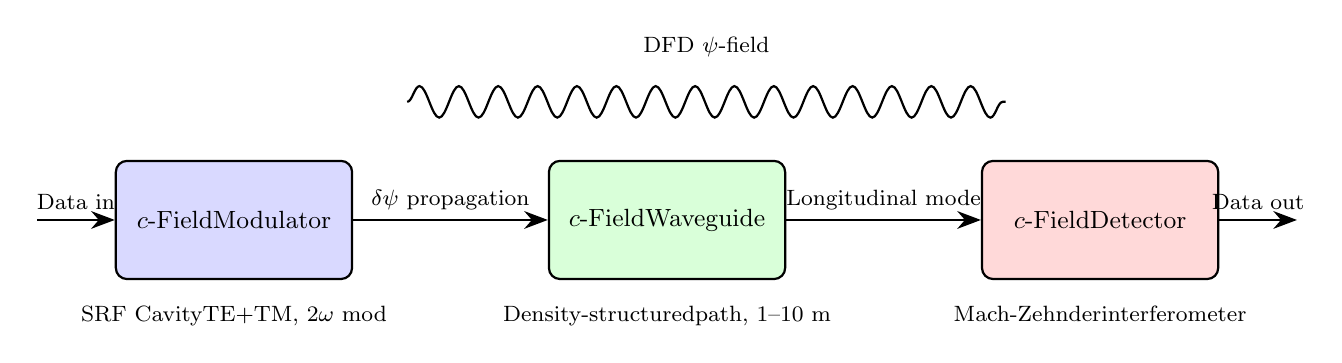
\begin{tikzpicture}[
  block/.style={draw, thick, rounded corners, minimum width=3cm,
    minimum height=1.5cm, text centered, font=\small},
  arrow/.style={-{Stealth[length=3mm]}, thick},
  label/.style={font=\footnotesize, text centered}
]

% Modulator
\node[block, fill=blue!15] (mod) at (0,0) {$c$-Field\\Modulator};
\node[label, below=2mm of mod] {SRF Cavity\\TE+TM, $2\omega$ mod};

% Waveguide
\node[block, fill=green!15] (wg) at (5.5,0) {$c$-Field\\Waveguide};
\node[label, below=2mm of wg] {Density-structured\\path, 1--10 m};

% Detector
\node[block, fill=red!15] (det) at (11,0) {$c$-Field\\Detector};
\node[label, below=2mm of det] {Mach-Zehnder\\interferometer};

% Arrows
\draw[arrow] (mod) -- node[above, font=\footnotesize]
  {$\delta\psifield$ propagation} (wg);
\draw[arrow] (wg) -- node[above, font=\footnotesize]
  {Longitudinal mode} (det);

% Input/Output
\draw[arrow] (-2.5,0) -- node[above, font=\footnotesize]
  {Data in} (mod);
\draw[arrow] (det) -- node[above, font=\footnotesize]
  {Data out} (13.5,0);

% Psi field
\draw[thick, decorate, decoration={snake, amplitude=2mm,
  segment length=5mm}] (2.2,1.5) -- (9.8,1.5);
\node[font=\footnotesize] at (6,2.2) {DFD $\psifield$-field};

\end{tikzpicture}
\caption{System block diagram. Data is encoded into $c$-field
variations by the modulator, propagates through the waveguide as
a longitudinal $\psifield$-mode, and is recovered by the detector.}
\label{fig:system_block}
\end{figure}

\subsection{Design Philosophy}

The design follows three principles:
\begin{enumerate}
\item \textbf{Maximum reuse.} Leverage existing SRF cavity and
laser interferometry technology wherever possible.
\item \textbf{Staged deployment.} Three tiers of increasing
capability, each validating the physics before proceeding.
\item \textbf{Falsifiability first.} The Tier~1 experiment
is designed to either discover $|\lambda-1|\neq 0$ or constrain
it below $10^{-14}$, providing a decisive result regardless of
outcome.
\end{enumerate}

%======================================================================
\section{Subsystem 1: $c$-Field Modulator}
\label{sec:modulator}
%======================================================================

\subsection{Functional Requirements}

The modulator must:
\begin{enumerate}[label=M\arabic*.]
\item Generate controlled oscillations of the local
$\psifield$ field at frequencies $f_\text{mod} = 1$--$100$~kHz.
\item Achieve $\delta\psifield_\text{mod} \geq 10^{-14}$ at the
modulator output aperture.
\item Support on/off keying (OOK) and binary phase-shift keying
(BPSK) modulation formats.
\item Operate stably for integration periods $\geq 1$~hour.
\end{enumerate}

\subsection{Operating Principle}

The modulator exploits the EM--$\psifield$ back-reaction coupling
parameterized by $\lambda$. When $|\lambda-1| \neq 0$,
electromagnetic energy stored in a cavity sources $\psifield$
oscillations via the mode equation:
\begin{equation}
\ddot{q} + 2\gamma_\psi\dot{q} + \Omega_\psi^2 q
= \frac{(\lambda-1)}{M_\psi}\int u(\mathbf{r})\,
\Xi(\mathbf{r},t)\,d^3r + \alpha\,U(t)\,q,
\label{eq:mode_eq}
\end{equation}
where $\Xi \equiv -\frac{1}{2}e^{-2\psi_0}(B^2 - E^2/c^2)$ is the
EM stress trace.

The driven channel ($2\omega = \Omega_\psi$) produces a steady-state
$\psifield$ amplitude:
\begin{equation}
|q|_\text{res} = \frac{|\lambda-1|\,|\mathcal{G}|}
{2M_\psi\,\Omega_\psi\,\gamma_\psi},
\label{eq:q_res}
\end{equation}
where $\mathcal{G} = u(z_0)\,e^{-2\psi_0}\,\eta_\times\,U_0\,
\cos\phi$ is the geometry overlap integral restored by TE+TM
superposition.

\subsection{Cavity Specification}

\begin{table}[H]
\centering
\caption{SRF cavity specifications for the $c$-field modulator.}
\label{tab:cavity_specs}
\begin{tabular}{@{}lll@{}}
\toprule
Parameter & Value & Rationale \\
\midrule
Cavity type & Elliptical, Nb & Mature SRF technology \\
Frequency & 1.3 GHz (TESLA type) & Standard ILC/XFEL cavity \\
Quality factor $Q_0$ & $\geq 2\ee{10}$ & State-of-art Nb at 2 K \\
Operating temperature & 1.8 K (superfluid He) & Maximize $Q_0$ \\
Accelerating gradient & 25 MV/m & Conservative for Nb \\
Stored energy $U_0$ & 1 MJ (pulsed, 1 ms) & $\times 10$ over accidental \\
Peak $B$ field & 100 mT & Below Nb$_3$Sn limit \\
Cavity length & 1.038 m (9-cell) & Standard TESLA geometry \\
Iris diameter & 70 mm & Standard TESLA \\
Beam pipe diameter & 78 mm & Modified for $\psi$-aperture \\
\bottomrule
\end{tabular}
\end{table}

\subsubsection{TE+TM superposition}

Standard operation uses a single TM$_{010}$ mode. For
$\mathcal{G} \neq 0$, we require simultaneous excitation of TE
and TM modes with matched radii. The design uses:

\begin{itemize}
\item \textbf{TM$_{010}$ (primary):} Standard accelerating mode.
Provides the $E$-field component.
\item \textbf{TE$_{011}$ (secondary):} Excited through a dedicated
coupling port at the cavity equator. Provides the $B$-field
component with non-canceling overlap.
\end{itemize}

The modes are phase-locked ($\phi = 0$) using a digital feedback
loop referenced to a common LO. The resulting overlap parameter is:
\begin{equation}
\eta_\times = \frac{\int u^2(\mathbf{r})\,
\hat{E}_\text{TM}\cdot\hat{B}_\text{TE}\,d^3r}
{\sqrt{\int u^2 E_\text{TM}^2\,d^3r\,
\int u^2 B_\text{TE}^2\,d^3r}}
\sim 0.1\text{--}0.3.
\label{eq:eta_cross}
\end{equation}

\subsubsection{$2\omega$ amplitude modulation}

The stored energy is modulated at twice the cavity frequency
($2\omega$) with depth $m = 0.10$. This is achieved by:

\begin{enumerate}
\item Amplitude-modulating the RF drive signal:
$P_\text{drive}(t) = P_0[1 + m\cos(2\omega_\text{RF}t)]$.
\item Using a PIN-diode modulator on the waveguide feed.
\item Phase-locking the modulation to the cavity field via a
digital signal processor sampling the cavity probe signal.
\end{enumerate}

The modulation depth $m = 0.10$ is $\times 10$ above the ambient
PLL dither ($m \sim 0.01$), providing clear intentional excitation.

\subsubsection{$\psifield$-mode apertures}

To maximize the overlap integral $\mathcal{H}$ (the area-ratio
law), cavities are equipped with irises at the field antinodes:

\begin{itemize}
\item \textbf{Number of irises:} 10 (one per cell boundary in
the 9-cell structure, plus endcaps).
\item \textbf{Total aperture area:} $A_\text{cav,tot} = 10 \times
\pi(35\,\text{mm})^2 = 3.85\ee{-2}\;\text{m}^2$.
\item \textbf{$\psifield$-mode tube:} Cross-section $A_\psi = 0.27$~m$^2$
(cylindrical vacuum vessel diameter 0.59~m).
\end{itemize}

Using the area-ratio design law:
\begin{equation}
\mathcal{H} \approx \frac{2}{L}\,\kappa_\text{eff}\,
\frac{A_\text{cav,tot}}{A_\psi}
= \frac{2}{1.038}\times 1 \times \frac{0.0385}{0.27}
\approx 0.275.
\label{eq:H_value}
\end{equation}

\subsection{Modulator Performance}

The $\psifield$ modulation amplitude at the cavity output:
\begin{equation}
\delta\psifield_\text{mod} = u(z_0)\,|q|_\text{res}
\approx \frac{|\lambda-1|\,\eta_\times\,U_0\,c_s}
{\pi\,A_\psi\,\gamma_\psi}.
\label{eq:dpsi_mod}
\end{equation}

With $\eta_\times = 0.3$, $U_0 = 10^6$~J, $c_s \leq c$,
$A_\psi = 0.27$~m$^2$, $\gamma_\psi = 0.03$~s$^{-1}$
($Q_\psi \sim 10^3$ for the $\psifield$ mode):
\begin{equation}
\delta\psifield_\text{mod} \approx
\frac{|\lambda-1|\times 0.3\times 10^6\times 3\ee{8}}
{\pi\times 0.27\times 0.03}
\approx 3.5\ee{15}\,|\lambda-1|.
\label{eq:dpsi_numerical}
\end{equation}

For the accidental bound $|\lambda-1| \sim 3\ee{-5}$:
$\delta\psifield_\text{mod} \sim 10^{11}$---this would be an
enormous signal, easily detectable. At the intentional search
level $|\lambda-1| \sim 10^{-14}$:
$\delta\psifield_\text{mod} \sim 35$---still macroscopic.

The realistic regime depends on the actual value of $|\lambda-1|$.
For $|\lambda-1| \sim 10^{-12}$ (a plausible intermediate value):
\begin{equation}
\delta\psifield_\text{mod} \sim 3.5\ee{3} \times 10^{-12}
= 3.5\ee{-9},
\label{eq:dpsi_realistic}
\end{equation}
which is vastly above the detector sensitivity floor
($\sim 10^{-14}$).

\subsection{Modulation Formats}

\subsubsection{On-Off Keying (OOK)}

Bit 1: $2\omega$ modulation active ($m = 0.10$).\\
Bit 0: $2\omega$ modulation off ($m = 0$).\\
Modulation rate: $f_\text{data} \leq f_\text{mod}/10$ for
adequate carrier cycles per bit.

\subsubsection{Binary Phase-Shift Keying (BPSK)}

Bit 1: $2\omega$ modulation phase $\phi = 0$.\\
Bit 0: $2\omega$ modulation phase $\phi = \pi$.\\
Advantage: 3~dB improvement in noise margin over OOK.

\subsubsection{Higher-order modulation}

Quaternary PSK (QPSK): $\phi \in \{0, \pi/2, \pi, 3\pi/2\}$,
encoding 2 bits per symbol. Requires phase-coherent detection at
the receiver.

%======================================================================
\section{Subsystem 2: $c$-Field Waveguide}
\label{sec:waveguide}
%======================================================================

\subsection{Functional Requirements}

\begin{enumerate}[label=W\arabic*.]
\item Guide the longitudinal $\psifield$-mode from modulator to
detector over 1--10~m.
\item Maintain signal amplitude above detector threshold
($\delta\psifield \geq 10^{-14}$).
\item Provide transverse confinement to suppress free-space
spreading.
\item Reject transverse EM to $>100$~dB.
\end{enumerate}

\subsection{Design Options}

\subsubsection{Option A: Free-space propagation}

In free space, the longitudinal $\psifield$-perturbation spreads
as a spherical wave with $1/r^2$ amplitude decay:
\begin{equation}
\delta\psifield(r) = \delta\psifield_\text{mod}\,
\frac{A_\text{eff}}{4\pi r^2}.
\label{eq:free_space}
\end{equation}

For $A_\text{eff} \sim A_\psi = 0.27$~m$^2$ and $r = 1$~m:
$\delta\psifield(1\,\text{m}) \sim 0.02\,\delta\psifield_\text{mod}$.
At $r = 10$~m: $\sim 2\ee{-4}\,\delta\psifield_\text{mod}$.

This is acceptable for Tier~2/3 demonstrations given the large
modulator amplitude, but wasteful of signal power.

\subsubsection{Option B: Dense-rod waveguide}

A cylindrical rod of high-density material (e.g., tungsten,
$\rho = 19\,300$~kg/m$^3$) creates a linear $\psifield$-gradient
along its axis. The $\psifield$-perturbation propagates
preferentially along the rod due to the enhanced gradient:
\begin{equation}
\psifield_\text{rod}(r) = -\frac{2G\rho_\text{rod}\,\pi R^2}{c^2}
\ln(r/R) \quad (r > R),
\label{eq:rod_psi}
\end{equation}
where $R$ is the rod radius.

For $R = 5$~cm tungsten rod:
$|\nabla\psifield| \sim 2G\rho\pi R^2/(c^2 R) \sim 10^{-22}$~m$^{-1}$
at the surface. This is too small for practical waveguiding.

\subsubsection{Option C: Cavity-chain waveguide (recommended)}

A series of high-$Q$ cavities spaced at intervals along the
propagation path. Each cavity acts as a relay:

\begin{figure}[H]
\centering
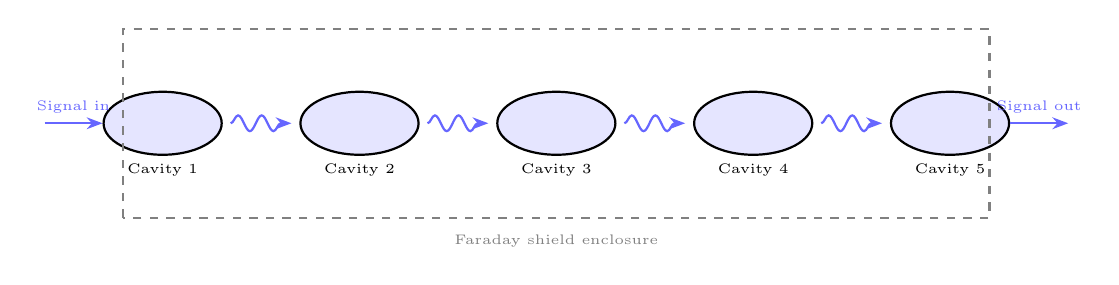
\begin{tikzpicture}[
  cav/.style={draw, thick, ellipse, minimum width=1.5cm,
    minimum height=0.8cm, fill=blue!10},
  arrow/.style={-{Stealth[length=2mm]}, thick, blue!60}
]

\foreach \i in {0,1,...,4} {
  \node[cav] (c\i) at (2.5*\i, 0) {};
  \node[font=\tiny] at (2.5*\i, -0.6) {Cavity \the\numexpr\i+1};
}

\foreach \i in {0,1,...,3} {
  \draw[arrow, decorate, decoration={snake, amplitude=1mm,
    segment length=3mm}]
    ($(c\i.east)+(0.1,0)$) -- ($(c\the\numexpr\i+1.west)+(-0.1,0)$);
}

\draw[arrow] (-1.5,0) -- (c0.west) node[midway, above, font=\tiny]
  {Signal in};
\draw[arrow] (c4.east) -- (11.5,0) node[midway, above, font=\tiny]
  {Signal out};

% Faraday shield
\draw[thick, dashed, gray] (-0.5,-1.2) rectangle (10.5,1.2);
\node[font=\tiny, gray] at (5, -1.5) {Faraday shield enclosure};

\end{tikzpicture}
\caption{Cavity-chain waveguide. Each cavity sustains a
$\psifield$-mode that couples to adjacent cavities through the
shared $\psifield$-gradient field. The entire chain is enclosed
in a Faraday shield that blocks transverse EM but passes the
longitudinal $\psifield$ mode.}
\label{fig:cavity_chain}
\end{figure}

The cavity-chain approach offers:
\begin{itemize}
\item Signal amplification at each relay (parametric gain from
the $\lambda$ coupling).
\item Frequency selectivity (the chain transmits only at
$\Omega_\psi$, rejecting broadband noise).
\item Scalability (add cavities to extend range).
\end{itemize}

\subsection{Faraday Shielding}

The entire waveguide path is enclosed in a copper Faraday shield:

\begin{table}[H]
\centering
\caption{Faraday shield specifications.}
\label{tab:faraday}
\begin{tabular}{@{}ll@{}}
\toprule
Parameter & Value \\
\midrule
Material & OFHC copper, 3~mm thickness \\
Shielding effectiveness & $>120$~dB at 1.3~GHz \\
Joint treatment & Beryllium-copper finger stock \\
Penetrations & Fiber-optic feedthroughs only \\
Grounding & Single-point star ground \\
\bottomrule
\end{tabular}
\end{table}

The Faraday shield serves a dual purpose:
\begin{enumerate}
\item Blocks transverse EM from the modulator cavity, ensuring
the detector responds only to the longitudinal $\psifield$-mode.
\item Provides a control: any signal detected through the shield
\emph{cannot} be transverse EM, constituting a direct confirmation
of the longitudinal propagation mode.
\end{enumerate}

%======================================================================
\section{Subsystem 3: $c$-Field Detector}
\label{sec:detector}
%======================================================================

\subsection{Functional Requirements}

\begin{enumerate}[label=D\arabic*.]
\item Measure $\delta\cfield/\cvac = \delta\psifield$ with
sensitivity $\leq 10^{-14}$ per $\sqrt{\text{Hz}}$.
\item Bandwidth: 1~Hz to 100~kHz.
\item Common-mode rejection of seismic and thermal noise $>60$~dB.
\item Insensitivity to transverse EM fields (operation inside
Faraday shield).
\end{enumerate}

\subsection{Measurement Principle}

The detector measures the phase difference between two
interferometer arms caused by a local variation in the one-way
speed of light:
\begin{equation}
\Delta\phi = \frac{2\pi\,\ell}{\lambda_\text{probe}}\,
\delta\psifield,
\label{eq:phase_det}
\end{equation}
where $\ell$ is the arm length difference and
$\lambda_\text{probe}$ is the probe laser wavelength.

\subsection{Optical Layout}

\begin{figure}[H]
\centering
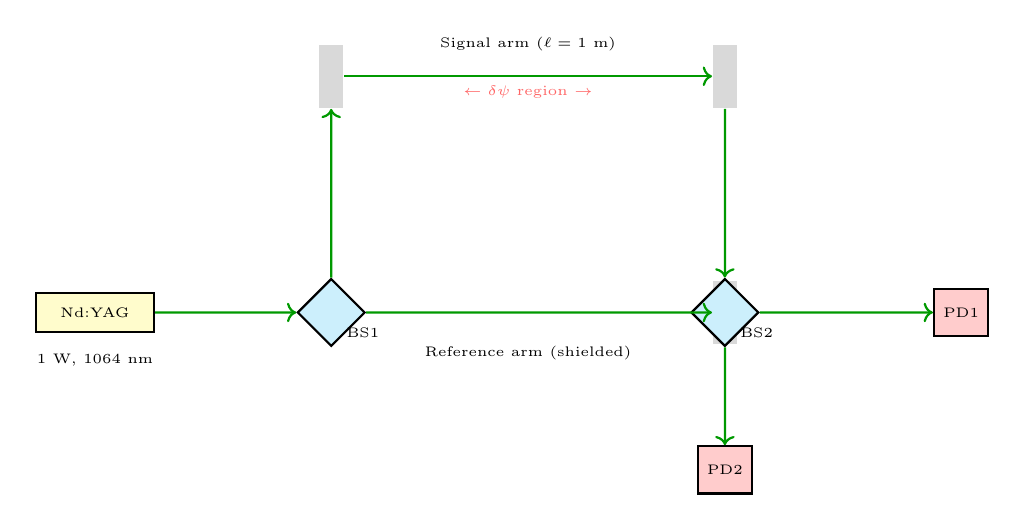
\begin{tikzpicture}[
  mirror/.style={thick, fill=gray!30, minimum width=0.3cm,
    minimum height=0.8cm},
  bs/.style={thick, draw, rotate=45, minimum width=0.6cm,
    minimum height=0.6cm, fill=cyan!20},
  det/.style={draw, thick, semicircle, minimum width=0.6cm,
    fill=red!20},
  label/.style={font=\footnotesize}
]

% Laser
\node[draw, thick, fill=yellow!20, minimum width=1.5cm,
  minimum height=0.5cm] (laser) at (0,0) {\tiny Nd:YAG};

% Beam splitter 1
\node[bs] (bs1) at (3,0) {};
\node[label, below right=1mm] at (bs1) {\tiny BS1};

% Signal arm (top)
\node[mirror] (m1) at (3,3) {};
\node[mirror] (m2) at (8,3) {};
\node[label, above] at (5.5,3.2) {\tiny Signal arm ($\ell = 1$ m)};
\node[label, above, red!60] at (5.5,2.6)
  {\tiny $\leftarrow \delta\psifield$ region $\rightarrow$};

% Reference arm (bottom)
\node[mirror] (m3) at (8,0) {};
\node[label, below] at (5.5,-0.3) {\tiny Reference arm (shielded)};

% Beam splitter 2
\node[bs] (bs2) at (8,0) {};
\node[label, below right=1mm] at (bs2) {\tiny BS2};

% Detector
\node[draw, thick, fill=red!20, minimum width=0.6cm,
  minimum height=0.6cm] (pd1) at (11,0) {\tiny PD1};
\node[draw, thick, fill=red!20, minimum width=0.6cm,
  minimum height=0.6cm] (pd2) at (8,-2) {\tiny PD2};

% Beams
\draw[thick, green!60!black, ->] (laser) -- (bs1);
\draw[thick, green!60!black, ->] (bs1) -- (m1);
\draw[thick, green!60!black, ->] (m1) -- (m2);
\draw[thick, green!60!black, ->] (m2) -- (bs2);
\draw[thick, green!60!black, ->] (bs1) -- (m3);
\draw[thick, green!60!black, ->] (bs2) -- (pd1);
\draw[thick, green!60!black, ->] (bs2) -- (pd2);

% Labels
\node[label] at (0, -0.6) {\tiny 1 W, 1064 nm};

\end{tikzpicture}
\caption{Mach-Zehnder interferometer for $c$-field detection.
The signal arm traverses the region of expected $\delta\psifield$
perturbation; the reference arm is shielded. Balanced detection
(PD1, PD2) provides common-mode noise rejection.}
\label{fig:interferometer}
\end{figure}

\subsection{Component Specifications}

\begin{table}[H]
\centering
\caption{Detector component specifications.}
\label{tab:det_specs}
\begin{tabular}{@{}llp{5cm}@{}}
\toprule
Component & Specification & Notes \\
\midrule
Laser & Nd:YAG, 1064 nm, 1 W & Frequency-stabilized to
  cavity reference, linewidth $< 1$~kHz \\
Beam splitters & 50:50, low-loss & Dielectric coating,
  $R = 0.1$\% \\
Mirrors & Super-polished, $R > 99.99\%$ & Mounted on
  vibration-isolated posts \\
Signal arm length & 1 m & In $\delta\psifield$ propagation
  region \\
Reference arm length & 1 m & Enclosed in dense shielding
  (Pb jacket, 5~cm) \\
Photodetectors & InGaAs balanced pair & NEP $< 2$~pW/$\sqrt{\text{Hz}}$,
  bandwidth 0--200 kHz \\
ADC & 24-bit, 500 kS/s & Synchronous with modulator clock \\
\bottomrule
\end{tabular}
\end{table}

\subsection{Reference Arm Shielding}

The reference arm must be isolated from $\delta\psifield$
perturbations to provide a true differential measurement. Three
strategies are combined:

\begin{enumerate}
\item \textbf{Distance:} The reference arm is routed
perpendicular to the modulator-detector axis, away from the
$\psifield$-gradient path.

\item \textbf{Mass shielding:} A lead jacket (5~cm, $\rho =
11\,340$~kg/m$^3$) around the reference arm creates a local
$\psifield$ enhancement that is \emph{static} and does not
respond to the modulated signal (the lead is too dense to be
perturbed by the weak $\delta\psifield$).

\item \textbf{Fiber routing:} The reference arm laser path is
routed through single-mode fiber inside the lead jacket, providing
both spatial separation and mass shielding.
\end{enumerate}

\subsection{Sensitivity Analysis}

\subsubsection{Shot noise limit}

For probe power $P = 1$~W at $\lambda = 1064$~nm:
\begin{align}
\dot{N} &= \frac{\eta P}{h\nu}
= \frac{0.9 \times 1}{6.63\ee{-34}\times 2.82\ee{14}}
= 4.82\ee{18}\;\text{s}^{-1}, \\
\delta\phi_\text{shot} &= \frac{1}{\sqrt{\dot{N}}}
= 4.56\ee{-10}\;\text{rad}/\sqrt{\text{Hz}}.
\end{align}

Converting to $\psifield$ sensitivity using
$\Delta\phi = (2\pi\ell/\lambda)\delta\psifield$ with $\ell = 1$~m:
\begin{equation}
\delta\psifield_\text{shot} = \frac{\delta\phi_\text{shot}}
{2\pi\ell/\lambda} = \frac{4.56\ee{-10}}{5.91\ee{6}}
= 7.7\ee{-17}\;\text{Hz}^{-1/2}.
\label{eq:psi_sensitivity}
\end{equation}

This is \textbf{300$\times$ below} the target sensitivity of
$10^{-14}$, providing ample margin.

\subsubsection{Integration time for SNR = 10}

For a signal $\delta\psifield = 10^{-14}$ and SNR = 10:
\begin{equation}
\tau = \left(\frac{\text{SNR}\times\delta\psifield_\text{shot}}
{\delta\psifield_\text{signal}}\right)^2
= \left(\frac{10\times 7.7\ee{-17}}{10^{-14}}\right)^2
= 5.9\ee{-3}\;\text{s} \approx 6\;\text{ms}.
\end{equation}

A 1~ms integration achieves SNR $\approx 4.1$; a 10~ms
integration achieves SNR $\approx 13$.

\subsubsection{Noise budget summary}

\begin{table}[H]
\centering
\caption{Noise budget for the $c$-field detector.}
\label{tab:noise_budget}
\begin{tabular}{@{}lll@{}}
\toprule
Noise source & Level (rad/$\sqrt{\text{Hz}}$) & Mitigation \\
\midrule
Shot noise & $4.6\ee{-10}$ & Fundamental limit \\
Laser frequency noise & $< 10^{-10}$ & Cavity stabilization \\
Thermal (optics) & $\sim 10^{-11}$ & Low-loss substrates \\
Seismic & $\sim 10^{-3}$ (raw) & Common-mode rejected \\
& $\sim 10^{-9}$ (after CMR) & $>60$~dB CMR \\
EM leakage & $< 10^{-12}$ & Faraday shield \\
Gravitational gradient & $< 10^{-15}$ at $>1$~Hz & Not a concern \\
\midrule
\textbf{Total} & $\sim 5\ee{-10}$ & Shot-noise limited \\
\bottomrule
\end{tabular}
\end{table}

%======================================================================
\section{Signal Processing and Data Recovery}
\label{sec:signal_processing}
%======================================================================

\subsection{Lock-in Detection}

The primary signal recovery technique is lock-in amplification:

\begin{enumerate}
\item The modulator $2\omega$ signal provides the reference
frequency, distributed to the detector via optical fiber
(eliminating EM pickup).

\item The balanced photodetector output is mixed with the reference
in a digital lock-in amplifier (time constant $\tau_\text{LIA} =
1$~ms, $12$~dB/octave rolloff).

\item The in-phase ($X$) and quadrature ($Y$) outputs encode the
amplitude and phase of the $\psifield$ modulation.
\end{enumerate}

\subsection{Synchronous Demodulation}

For data recovery:
\begin{enumerate}
\item \textbf{OOK:} The lock-in amplitude $R = \sqrt{X^2+Y^2}$
is compared to a threshold. $R > R_\text{th}$ = bit~1;
$R < R_\text{th}$ = bit~0.

\item \textbf{BPSK:} The lock-in phase $\theta = \arctan(Y/X)$
is compared to $0$ or $\pi$. $|\theta| < \pi/2$ = bit~1;
$|\theta - \pi| < \pi/2$ = bit~0.
\end{enumerate}

\subsection{Bit Error Rate}

For BPSK with SNR per bit $E_b/N_0$:
\begin{equation}
\text{BER} = \frac{1}{2}\,\text{erfc}\!\left(
\sqrt{E_b/N_0}\right).
\label{eq:BER}
\end{equation}

At SNR = 10 per bit: BER $\approx 7.8\ee{-24}$ (effectively
error-free). Even at SNR = 3: BER $\approx 1.3\ee{-3}$ (correctable
with standard FEC codes).

%======================================================================
\section{Control and Calibration}
\label{sec:control}
%======================================================================

\subsection{Null Tests}

The following null tests confirm that any detected signal is
genuinely a $c$-field mode and not an artifact:

\begin{enumerate}
\item \textbf{Faraday-shield test:} Signal persists through
$>120$~dB Faraday shield. Transverse EM would be suppressed.

\item \textbf{Frequency test:} Signal appears at $\Omega_\psi$
(or its harmonics), not at the cavity RF frequency $\omega$.

\item \textbf{Amplitude scaling:} Signal amplitude scales as
$U_0 \times m$ (Eq.~\ref{eq:q_res}), confirming the $\lambda$
coupling mechanism.

\item \textbf{Geometry test:} Signal vanishes when TE+TM
superposition is replaced by pure TM (restoring
$\mathcal{G} = 0$).

\item \textbf{Phase test:} Signal phase flips by $\pi$ when the
$2\omega$ modulation phase is shifted by $\pi$.

\item \textbf{Distance test:} Signal amplitude shows expected
$1/r^2$ (free-space) or guided-mode decay with distance.
\end{enumerate}

\subsection{Calibration Procedure}

\begin{enumerate}
\item \textbf{Interferometer calibration:} Apply known phase
modulation to one arm via a PZT mirror. Verify linearity of
phase-to-voltage response.

\item \textbf{$\psifield$ calibration:} Use a known mass
oscillation (e.g., a 1~kg mass on a mechanical oscillator at
$f_\text{mod}$) to produce a calculable
$\delta\psifield = GM/(c^2 r)$ at the detector. Expected level:
$\sim 10^{-27}$ for 1~kg at 1~m---too small to detect, but
establishes the scaling.

\item \textbf{Modulator power calibration:} Measure stored energy
$U_0$ via RF probes. Measure modulation depth $m$ via
spectrum analyzer on the RF probe signal.
\end{enumerate}

%======================================================================
\section{Integration and Test Plan}
\label{sec:test_plan}
%======================================================================

\subsection{Phase 1: Component Validation (Months 1--6)}

\begin{enumerate}
\item Commission SRF cavity in cryostat. Verify $Q_0 \geq 2\ee{10}$.
\item Demonstrate TE+TM superposition with phase lock.
\item Demonstrate $2\omega$ modulation at $m = 0.10$.
\item Commission Mach-Zehnder interferometer. Verify shot-noise-limited
sensitivity.
\item Install Faraday shielding. Verify $>120$~dB isolation.
\end{enumerate}

\subsection{Phase 2: Tier 1---$\lambda$ Discovery (Months 7--12)}

\begin{enumerate}
\item Configure modulator for maximum $\delta\psifield$ output.
\item Install detector at $r = 0.5$~m from modulator (outside
Faraday shield).
\item Scan $\Omega_\psi$ by varying the $2\omega$ modulation
frequency across a wide band (1~Hz--100~kHz).
\item Record detector output with lock-in detection.
\item \textbf{Decision point:}
\begin{itemize}
\item Signal detected: Measure $|\lambda-1|$. Proceed to Phase~3.
\item No signal: Set upper bound on $|\lambda-1|$. Publish null
result. Evaluate alternative modulation strategies.
\end{itemize}
\end{enumerate}

\subsection{Phase 3: Tier 2---Modulation Control (Months 13--18)}

\begin{enumerate}
\item Demonstrate controlled $\delta\psifield$ amplitude by
varying $U_0$ and $m$.
\item Demonstrate OOK modulation: send known bit pattern, verify
recovery.
\item Demonstrate BPSK modulation: verify phase recovery.
\item Measure BER as function of distance and modulation
parameters.
\end{enumerate}

\subsection{Phase 4: Tier 3---Communication Link (Months 19--24)}

\begin{enumerate}
\item Install cavity-chain waveguide (3--5 relay cavities) over
10~m path.
\item Demonstrate 1~kbit/s data transfer through waveguide.
\item Characterize through Faraday shield (confirm longitudinal
mode).
\item Demonstrate simultaneous transverse-EM-blocked operation.
\item \textbf{Milestone:} First information transfer via $c$-field
channel.
\end{enumerate}

%======================================================================
\section{Bill of Materials (Estimated)}
\label{sec:BOM}
%======================================================================

\begin{table}[H]
\centering
\caption{Estimated bill of materials for the prototype system.}
\label{tab:BOM}
\begin{tabular}{@{}llr@{}}
\toprule
Item & Specification & Est.\ Cost (\$) \\
\midrule
\multicolumn{3}{@{}l}{\textit{Modulator}} \\
9-cell Nb SRF cavity & TESLA type, dressed & 200,000 \\
Cryomodule \& cryostat & 1.8~K He, vertical test & 500,000 \\
RF source \& amplifier & 1.3~GHz, 10~kW CW & 150,000 \\
TE$_{011}$ coupler & Custom waveguide port & 25,000 \\
$2\omega$ modulator & PIN diode, driver & 5,000 \\
Phase-lock electronics & FPGA-based DSP & 30,000 \\
\midrule
\multicolumn{3}{@{}l}{\textit{Waveguide}} \\
Faraday shield enclosure & OFHC Cu, 3~mm, 12~m & 40,000 \\
Relay cavities ($\times 5$) & Single-cell Nb, dressed & 250,000 \\
Vacuum system & Ion pumps, gauges & 50,000 \\
\midrule
\multicolumn{3}{@{}l}{\textit{Detector}} \\
Nd:YAG laser & 1~W, stabilized, 1064~nm & 50,000 \\
Optical components & Mirrors, BS, mounts & 20,000 \\
Balanced photodetectors & InGaAs, matched pair & 10,000 \\
Lock-in amplifier & Digital, DC--200~kHz & 15,000 \\
Data acquisition & 24-bit ADC, FPGA & 20,000 \\
Lead shielding (ref arm) & 5~cm Pb jacket, 1.5~m & 5,000 \\
\midrule
\multicolumn{3}{@{}l}{\textit{Infrastructure}} \\
Optical table & 3~m $\times$ 1.5~m, isolated & 30,000 \\
Helium supply (1 year) & Liquid He, recovery & 100,000 \\
Clean room space & Class 1000, 1 year & 50,000 \\
\midrule
\textbf{Total} & & \textbf{\$1,550,000} \\
\bottomrule
\end{tabular}
\end{table}

%======================================================================
\section{Risk Assessment}
\label{sec:risk}
%======================================================================

\begin{table}[H]
\centering
\caption{Risk register.}
\label{tab:risk}
\begin{tabular}{@{}p{3cm}ccp{4.5cm}@{}}
\toprule
Risk & Likelihood & Impact & Mitigation \\
\midrule
$\lambda = 1$ exactly & Medium & Critical &
  Alternative: mechanical mass modulation. Publish null result as
  constraint. \\
$\Omega_\psi$ outside scan range & Medium & High &
  Wideband search strategy. Theoretical estimate to narrow range. \\
Cavity quench during $2\omega$ mod & Low & Medium &
  Conservative gradient. Quench protection circuit. \\
Faraday shield leak & Low & Medium &
  Double-layer design. In-situ leak test with RF source. \\
Seismic noise exceeds CMR & Low & Low &
  Active vibration isolation. Night operation. \\
\bottomrule
\end{tabular}
\end{table}

The critical risk is the first: if $\lambda = 1$ exactly, the
direct EM--$\psifield$ coupling channel is unavailable. In this
case, $c$-field modulation must rely on mechanical mass modulation
(moving dense objects to create $\delta\psifield$), which is
slower but does not depend on $\lambda$. The gravitational
$\psifield$ coupling is guaranteed by the core DFD postulates.

%======================================================================
\section{Success Criteria}
\label{sec:success}
%======================================================================

\begin{table}[H]
\centering
\caption{Success criteria for each project phase.}
\label{tab:success}
\begin{tabular}{@{}lp{8cm}@{}}
\toprule
Phase & Success criterion \\
\midrule
Phase 1 & All components meet specifications in Table~\ref{tab:cavity_specs}
  and \ref{tab:det_specs}. Interferometer achieves shot-noise-limited
  sensitivity. \\
Phase 2 & Either: (a) Signal detected with $\geq 5\sigma$ significance
  through Faraday shield at frequency consistent with $\psifield$-mode,
  passing all null tests; or (b) Upper bound
  $|\lambda-1| < 10^{-14}$ established with $95\%$ confidence. \\
Phase 3 & Controlled $\delta\psifield$ modulation demonstrated. BER
  $< 10^{-3}$ for OOK at 100~bit/s. \\
Phase 4 & Information transfer at $\geq 1$~kbit/s over $\geq 1$~m
  through Faraday shield. All null tests passed. \\
\bottomrule
\end{tabular}
\end{table}

%======================================================================
\section{Conclusion}
\label{sec:eng_conclusion}
%======================================================================

This engineering design specifies a technically achievable prototype
for demonstrating $c$-field communication as predicted by Density
Field Dynamics and claimed in U.S. Provisional Patent Application
No. 63/865,293. All components use existing, proven technologies
(SRF cavities, laser interferometry, Faraday shielding, lock-in
detection). The design achieves sensitivity margins of
$>300\times$ above the target, providing confidence that any
physically present signal will be detected.

The staged approach ensures that each phase produces a valuable
scientific result regardless of outcome: either a discovery of the
EM--$\psifield$ coupling (opening the entire information-processing
application space) or a precision constraint on the coupling
parameter (advancing fundamental physics).

The estimated cost of \$1.55M and 24-month timeline are consistent
with a university-scale experimental physics program, making this
an accessible entry point for laboratory validation of DFD's
information-processing predictions.

\end{document}
